\section*{Part 1}

Using the instructions provided in the project description, run memcached alone (i.e., no interference), and with each iBench source of interference (cpu, l1d, l1i, l2, llc, membw). For Part 1, you must use the following \texttt{mcperf} command, which varies the target QPS from 5000 to 80000 in increments of 5000 (and has a warm-up time of 2 seconds with the addition of \texttt{-w 2}):

\begin{verbatim}
$ ./mcperf -s MEMCACHED_IP --loadonly
$ ./mcperf -s MEMCACHED_IP -a INTERNAL_AGENT_IP  \
           --noload -T 8 -C 8 -D 4 -Q 1000 -c 8 -w 2 -t 5 \ 
           --scan 5000:80000:5000
\end{verbatim}

\noindent Repeat the run for each of the 7 configurations (without interference, and the 6 interference types) {\color{red} \textbf{at least 3 times}} (3 should be sufficient in this case), and collect the performance measurements (i.e. the \texttt{client-measure} VM output).

\noindent\textbf{\underline{Reminder:}} after you have collected all the measurements, make sure you \textbf{{\color{red}delete your cluster}}. Otherwise, you will easily use up the cloud credits. See the project description for instructions how to make sure your cluster is deleted.

%%%%%%%%%%%%%%%%%%%%%%%%%%%%%%%%%%%%%%%%%%%
%%% QUESTION 1A

\begin{enumerate}[label=(\alph*)]
    \setcounter{enumi}{0}

    \item Plot a line graph with the following stipulations:
    \begin{itemize}
        \item Queries per second (QPS) on the x-axis (the x-axis should range from 0 to 80K).\\
        (\textbf{note:} the actual achieved QPS, not the target QPS)
        \item 95th percentile latency on the y-axis (the y-axis should range from 0 to 6 ms).
        \item Label your axes.
        \item 7 lines, one for each configuration. Add a legend.
        \item State how many runs you averaged across and include error bars at each point in both dimensions.
        % \item The readability of your plot will be part of your grade.
    \end{itemize}
    
    % \textbf{The shape of the curves depends on many factors and may differ across groups. However, that does not imply that your solutions are wrong.} 
    
\end{enumerate}

\textbf{Answer:} % Here you place your solution.

\begin{figure}[H]
    \centering
    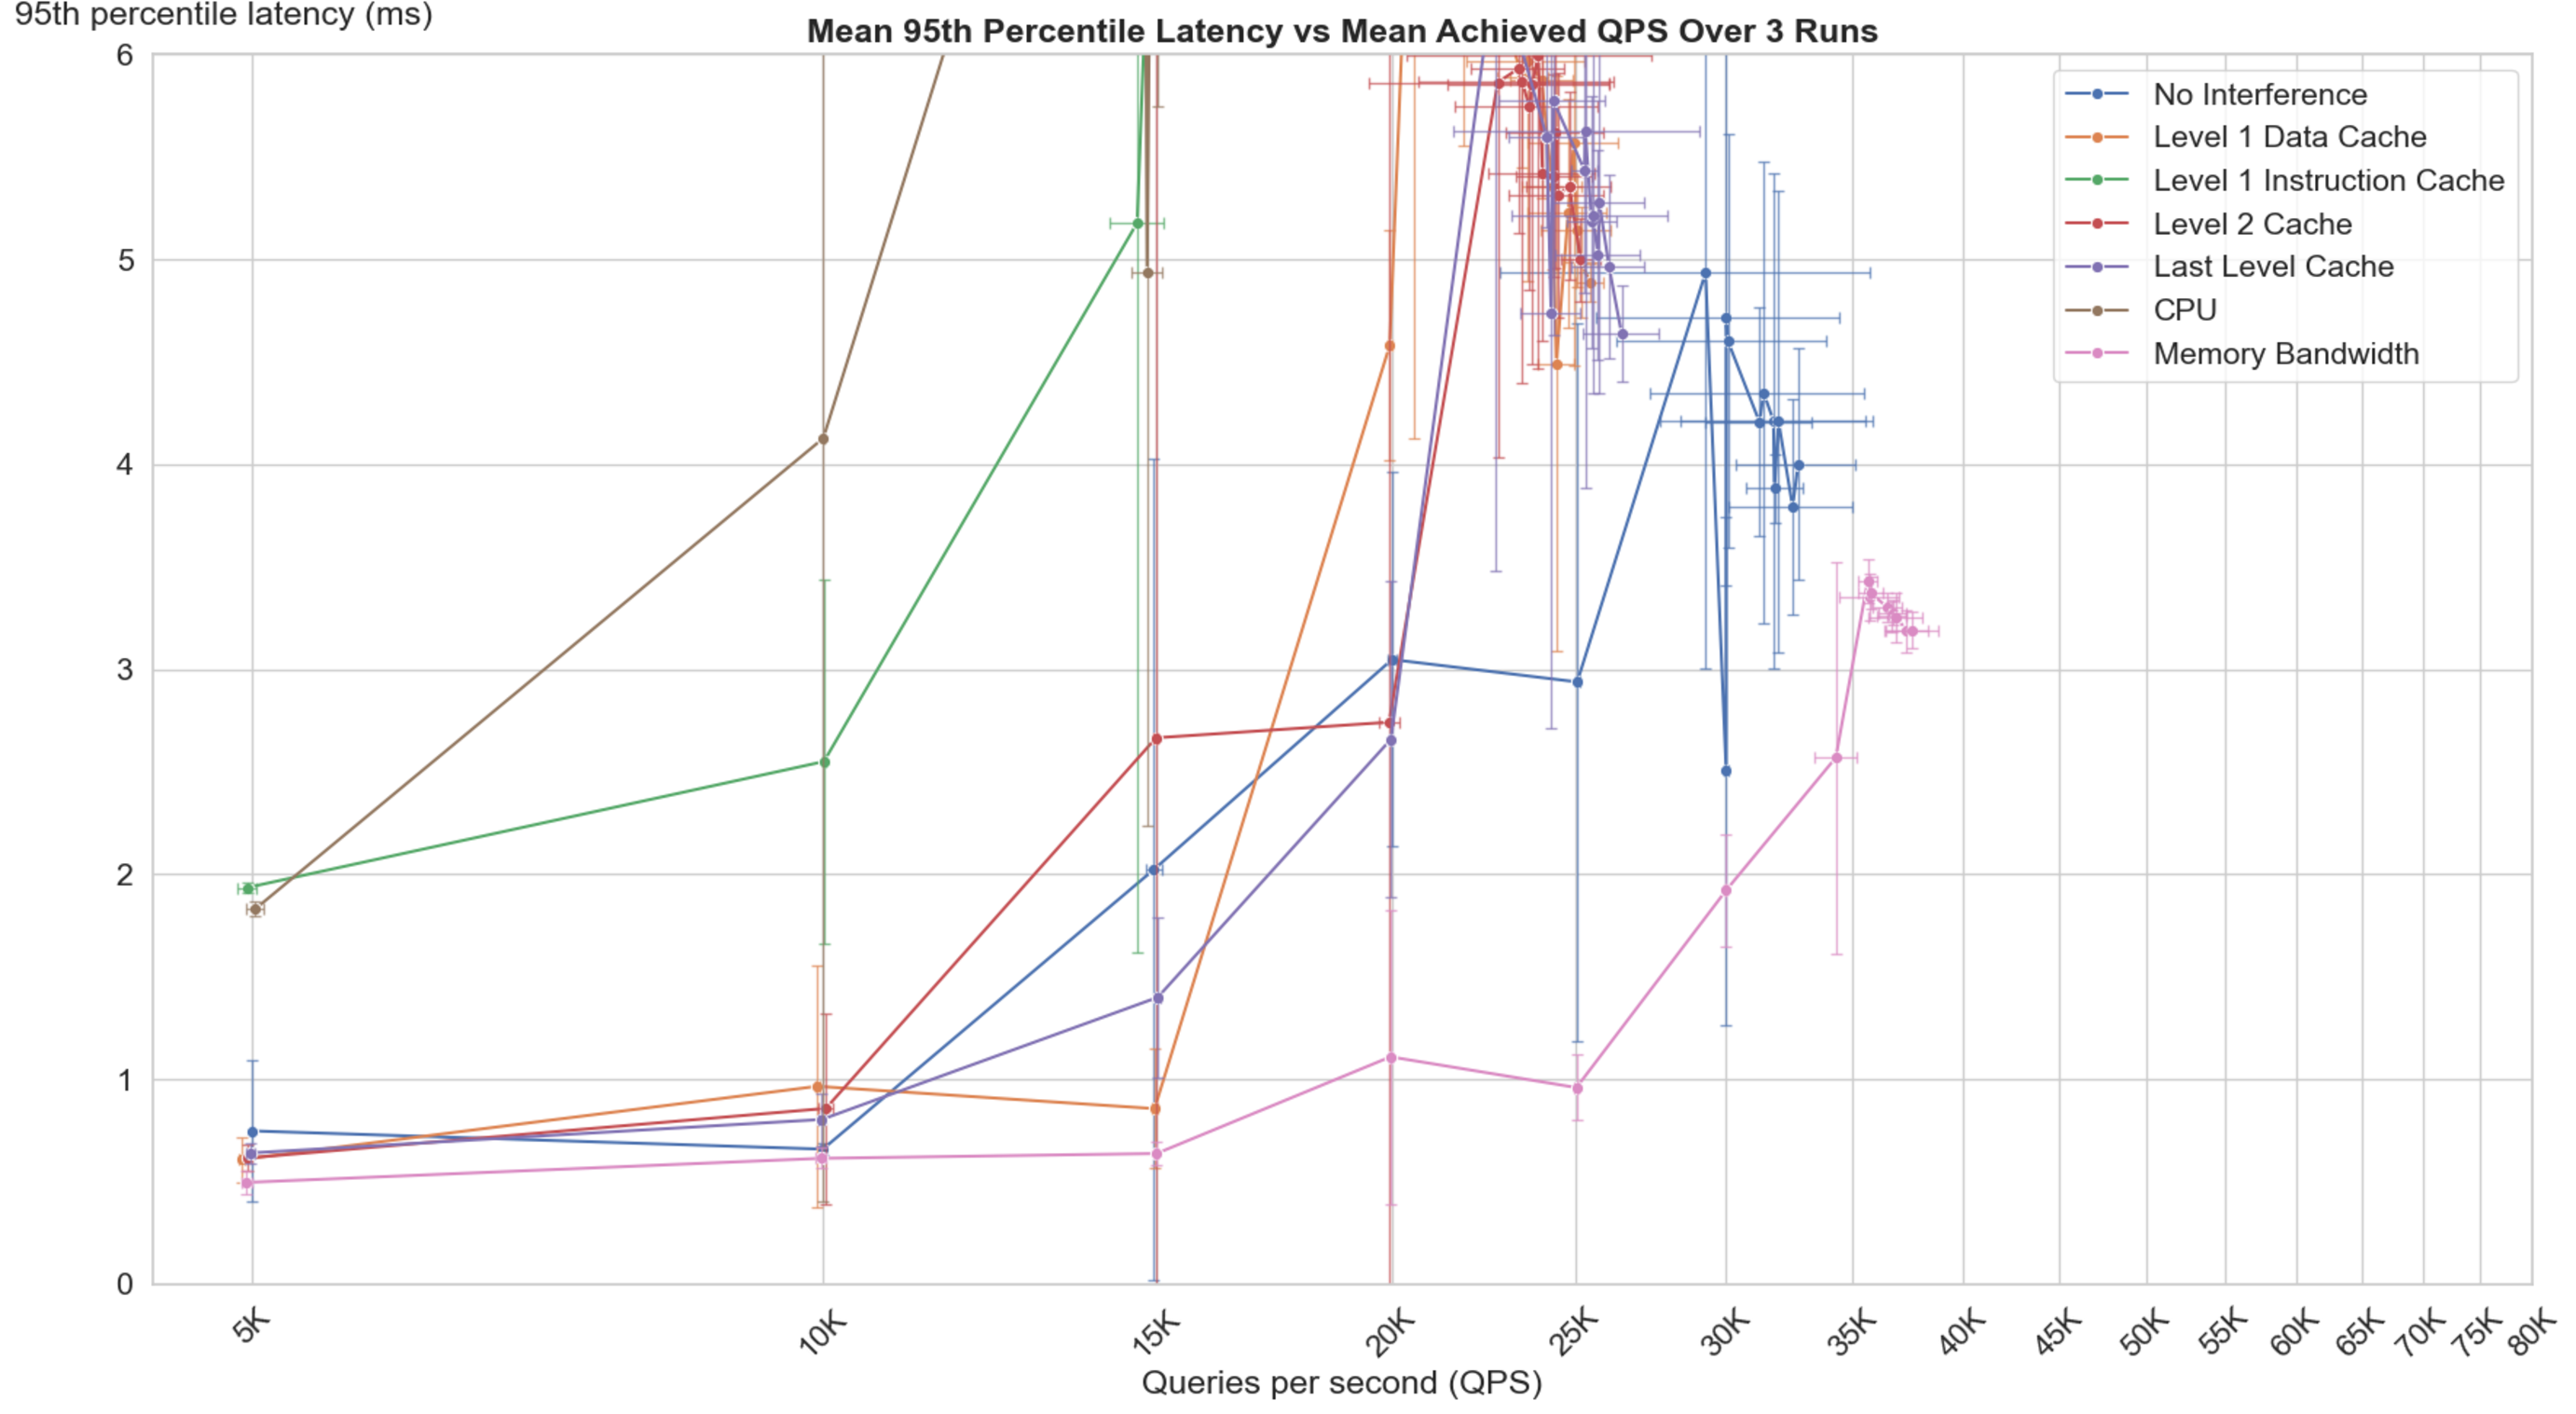
\includegraphics[width=1\linewidth]{report/figures/part1_required.pdf}
    \caption{95th percentile acoording to the achieved QPS, averaged over 3 runs, with the required plot limits from the tasks. QPS on logarithmic scale to distribute the measurements better over the plot.}
    \label{fig:part1_required}
\end{figure}

\begin{figure}[H]
    \centering
    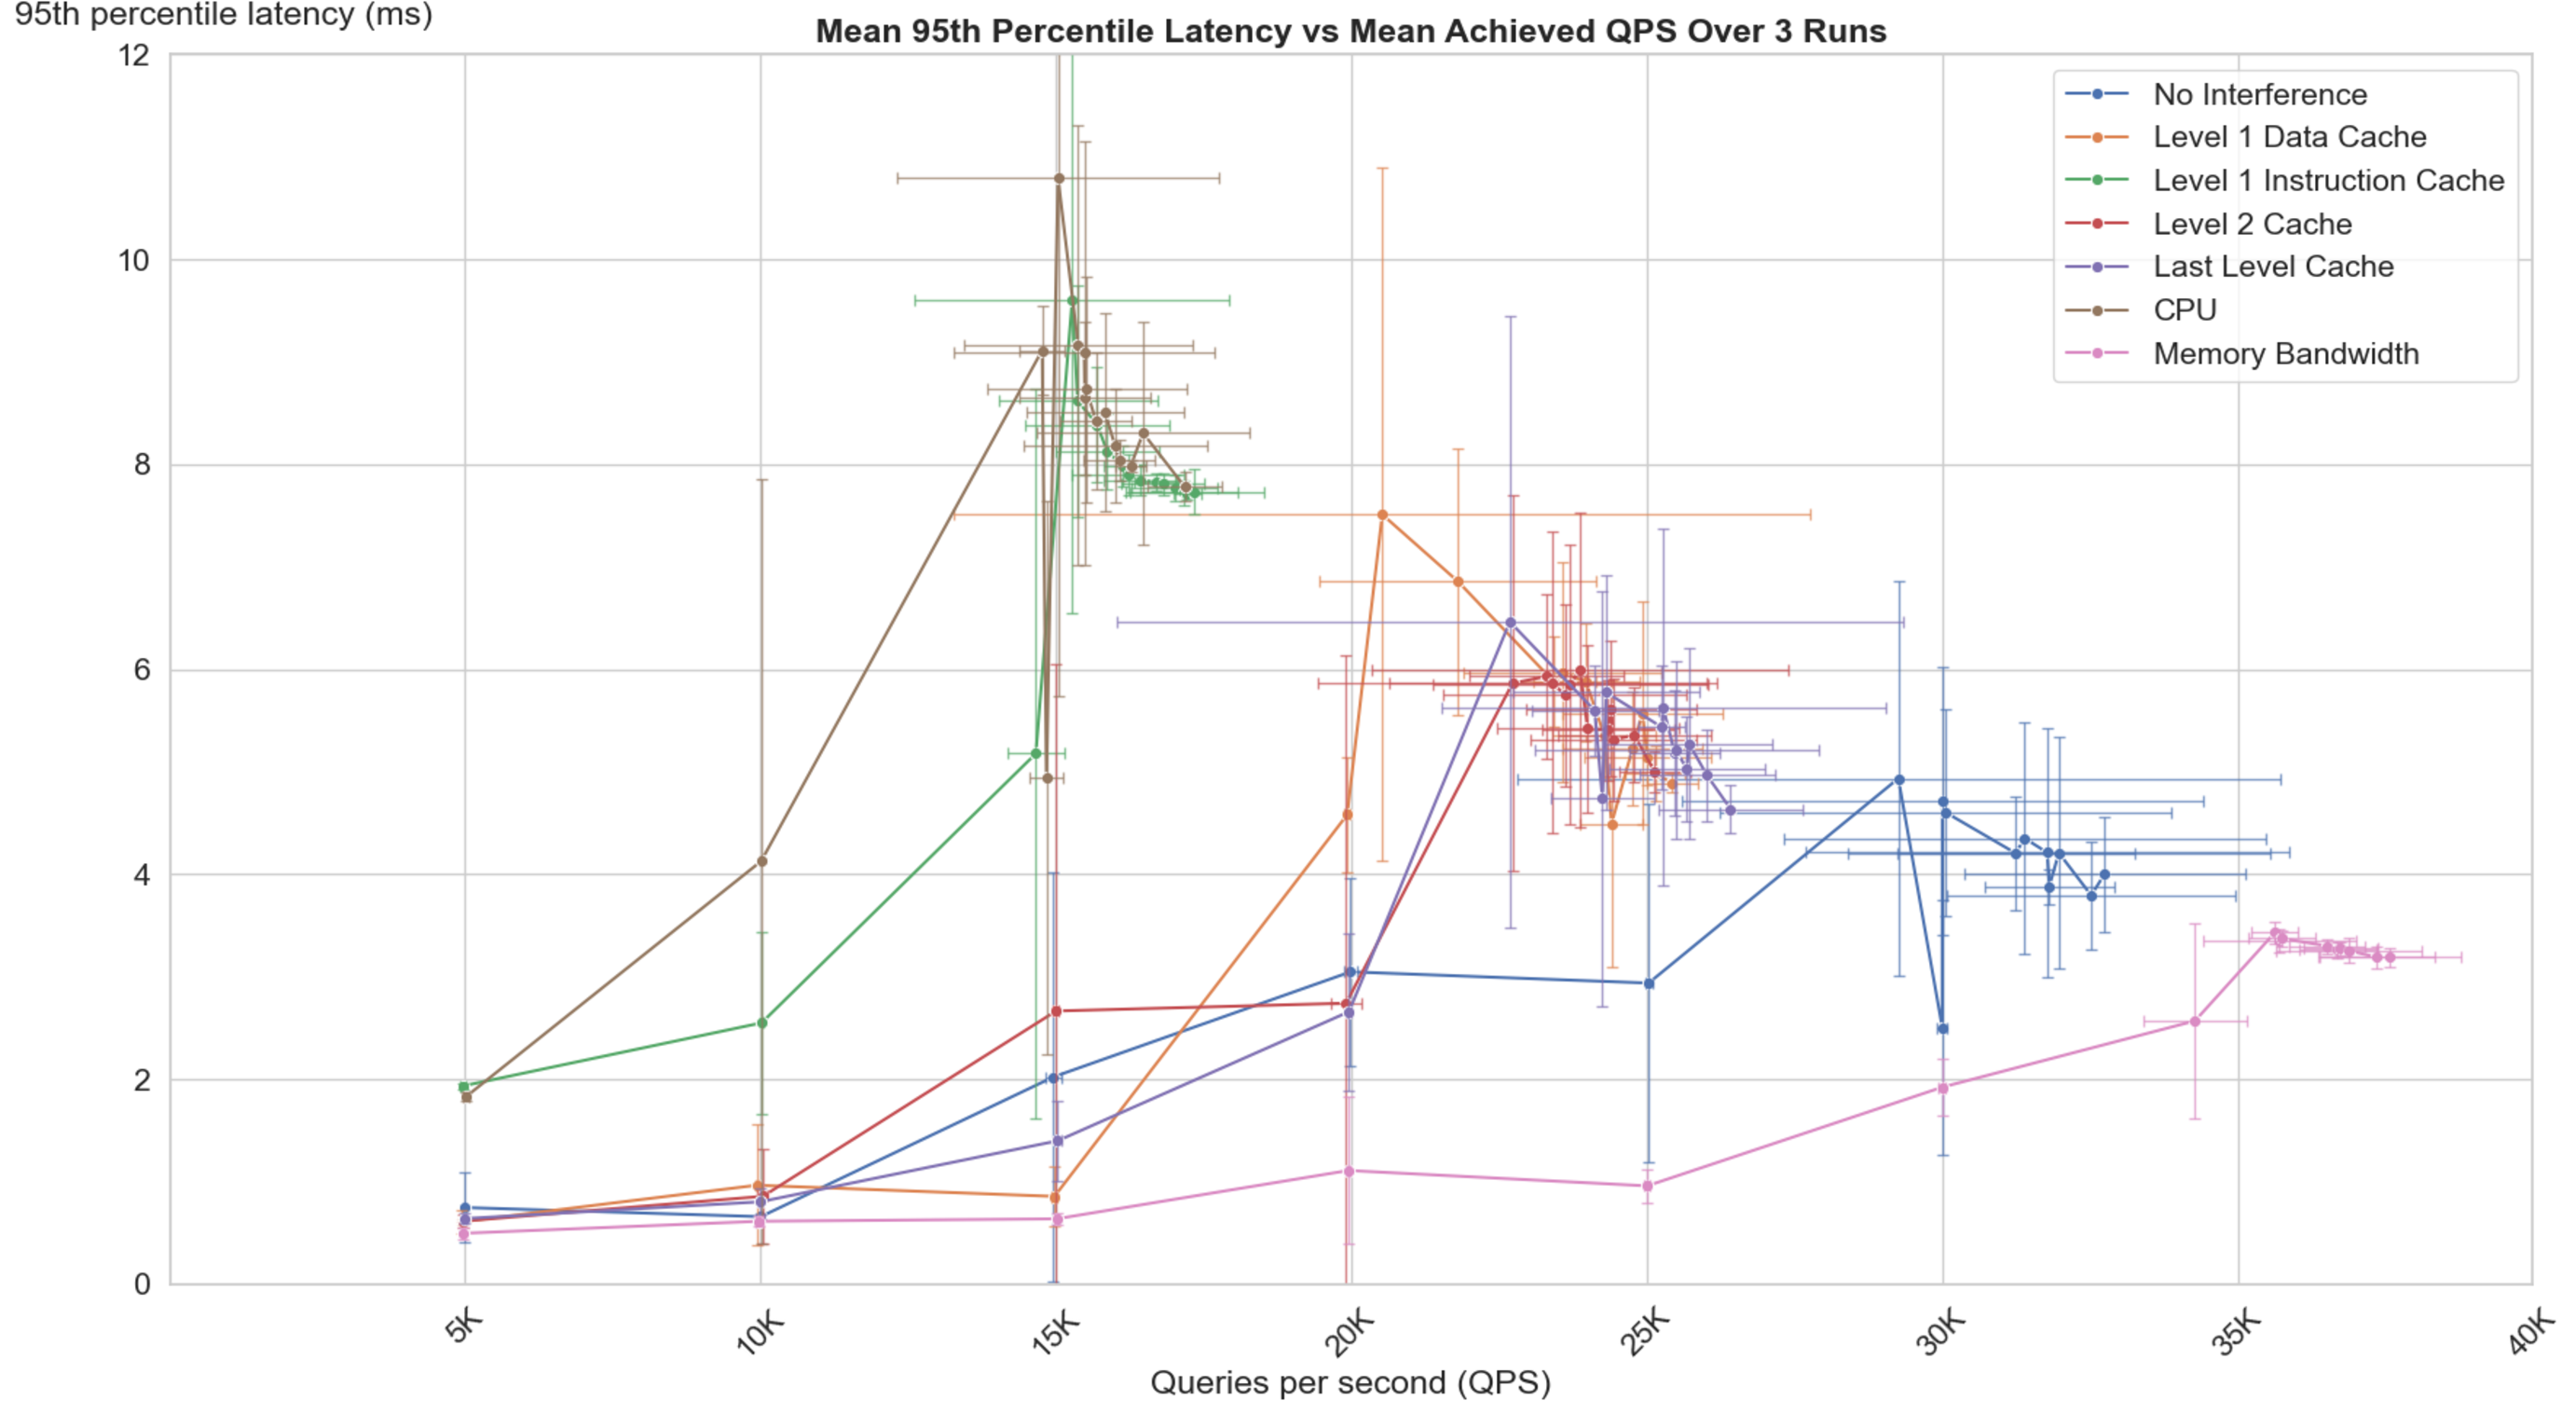
\includegraphics[width=1\linewidth]{report/figures/part1_adapted_axes.pdf}
    \caption{95th percentile acoording to the achieved QPS, averaged over 3 runs, with adjusted limits of the plot boundaries to show all measurements. Linear x-axis on the QPS measurements.}
    \label{fig:part1_adapted_axes}
\end{figure}

%%%%%%%%%%%%%%%%%%%%%%%%%%%%%%%%%%%%%%%%%%%
%%% QUESTION 1B

\begin{enumerate}[label=(\alph*)]
    \setcounter{enumi}{1}
    
    \item How is the tail latency and saturation point (the “knee in the curve”) of memcached affected by each type of interference? What is your reasoning for these effects? Briefly describe your hypothesis.
    
\end{enumerate}

\textbf{Answer:}
\begin{itemize}
    \item \texttt{ibench-cpu}: Large increase in tail latency (p95 exceeds $5ms$ at $12$K QPS) and very low saturation point ($\approx 15$K QPS).
    
    \textit{Explanation:} \texttt{memcached} and \texttt{ibench-cpu}'s benchmark run on core 0 and contend for the CPU; this increases queueing latency.
    
    \item \texttt{ibench-l1d}: Moderate latency increase; p95 stays at $\approx 1ms$ until $\approx 15$K QPS, then rises to $\approx 5ms$, saturating at $24$K QPS.
    
    \textit{Explanation:} \texttt{ibench-l1d} occupies core 0's L1 (data) cache rows. This gives \texttt{memcached} perpetual L1 cache misses, increasing service time and tail latency.

    \item \texttt{ibench-l1i}: Lowers the saturation point to $\approx 15$K QPS with p95 initially at $2ms$.
    
    \textit{Explanation:} \texttt{ibench-l1i} occupies/contends for core 0's L1 instruction cache. This cipples \texttt{memcached}'s CPU's fetch stage in its fetch–decode–execute cycle, almost as if its clockrate had slowed.

    \item \texttt{ibench-l2}: Moderate lowered saturation point at $25$K QPS – otherwise similar to the baseline.
    
    \textit{Explanation:} \texttt{ibench-l2} occupies core 0's L2 cache; this causes secondary cache misses in the event of an L1 cache miss. This affects p99 and p95 latency more than p50 latency due to the event being rarer (– not plotted, but p50 measurements confirm this).

    \item \texttt{ibench-llc}: Very similar to \texttt{ibench-l2} – slightly higher saturation point at $26$K.
    
    \textit{Explanation:} \texttt{ibench-llc} occupies core 0's L3 cache; for the same reasons as \texttt{ibench-l2}, this increases tail latency. 

    \item \texttt{ibench-membw}: Unexpectedly decreases tail latency roughly by half compared to the baseline, and improves the saturation point to $\approx 36$K. 
    
    \textit{Explanation:} One expects \texttt{ibench-membw} to be the least disruptive benchmark, since \texttt{memcached}'s working set fits in cache, however the decrease in tail latency is hard to explain; it could be due to noise and frequency scaling in the cloud provider.
\end{itemize}

%%%%%%%%%%%%%%%%%%%%%%%%%%%%%%%%%%%%%%%%%%%
%%% QUESTION 1C

\begin{enumerate}[label=(\alph*)]
    \setcounter{enumi}{2}
    \item Processor affinity:
    \begin{itemize}
        \item Explain the use of the \texttt{taskset} command in the container commands for memcached and iBench in the provided scripts.
        
        \textbf{Answer:} \texttt{taskset} enforces core affinity; it pins processes to CPUs. The benchmark uses it to core-pin \texttt{memcached} and \texttt{ibench}, which prevents the OS scheduler from reassigning them, to ensure controlled and predictable contention.
        \\

        \item Why do we run some of the iBench benchmarks on the same core as memcached and others on a different core? Give an explanation for each iBench benchmark.

        \textbf{Answer:} In order to occupy CPU, L1 and L2 caches, \texttt{ibench} must run on the same core, since those are local resources, unlike the L3 cache and memory. By occupying non-local resources from another core, one ensures, that local resources are not contended, i.e the L3 cache of core 0 is occupied from core 1 without contending with core 0's CPU. 
    \end{itemize}
    
\end{enumerate}

%%%%%%%%%%%%%%%%%%%%%%%%%%%%%%%%%%%%%%%%%%%
%%% QUESTION 1D
    
\begin{enumerate}[label=(\alph*)]
    \setcounter{enumi}{3}
    
    \item Assuming a service level objective (SLO) for memcached of up to 2~ms 95th percentile latency at 35K QPS, which iBench source of interference can safely be collocated with memcached without violating this SLO? Briefly explain your reasoning.
            
\end{enumerate}

\textbf{Answer:} \texttt{ibench-membw} is the only interference benchmark. All other benchmarks saturate before $35$K QPS.

%%%%%%%%%%%%%%%%%%%%%%%%%%%%%%%%%%%%%%%%%%%
%%% QUESTION 1E
    
\begin{enumerate}[label=(\alph*)]
    \setcounter{enumi}{4}
    
    \item In the lectures you have seen queueing theory. 
    \begin{itemize}
        \item Is the project experiment above (ignoring client measure) an open system or a closed system? Explain why.

        \textbf{Answer:} It's an open system, because \texttt{mcperf}'s generated request arrival rate is not limited by old requests being completed.
        \\

        \item What is the number of clients in the system? How did you find this number?

        \textbf{Answer:} 8 clients – that is what the \texttt{client-measure} VM's \texttt{mcperf} command specifies with \texttt{-c 8}:
        \begin{verbatim}
./mcperf -s MEMCACHED_IP -a \
    INTERNAL_AGENT_IP \
    --noload -T 8 -C 8 -D 4 -Q 1000 -c 8 -w 2 -t 5 \
    --scan 5000:80000:5000
\end{verbatim}

        \item Sketch a diagram of the queueing system modeling the experiment above. Give a brief explanation of the sketch.
   
        \textbf{Answer:} Because the \texttt{mcperf} command does not specify any custom inter-arrival distribution with \texttt{--iadist}, it uses the default exponential distribution. \texttt{memcached} runs on a single core. This means, that one can model the system as an $M/M/1$ open system.

        \begin{figure}[H]
            \centering
            \includegraphics[width=0.5\linewidth]{ex-1e-queue.png}
            \caption{Sketch of $M/M/1$ queueing system}
            \label{fig:placeholder}
        \end{figure}

        \item Provide an expression for the average response time of this system. Explain each term in this expression and match it to the parameters of the project experiment.
        
        \textbf{Answer:} $\mathbb{E} [w] = \frac{\mathbb{E} [n]}{\lambda} = \frac{\rho}{(1 - \rho)\lambda} = \frac{1}{(\mu - \lambda)}$ \\
        
        ($\lambda$ is QPS arrival rate, $\rho = \lambda/\mu$ is utilization, $\mu$ is \texttt{memcached}'s processing throughput. The first equality applies Little's Law; the second equality substitutes in the expected length of the $M/M/1$ Markov decision process.)
    \end{itemize}
            
\end{enumerate}

%%%%%%%%%%%%%%%%%%%%%%%%%%%%%%%%%%%%%%%%%%%
%%% QUESTION 1F
    
\begin{enumerate}[label=(\alph*)]
    \setcounter{enumi}{5}
    
    \item Below we ask you to do a theoretical cost analysis of the above experiments you ran and compare with the actual cost of your experiments, for which you will \textbf{need to track the total runtime} of the experiments, from deploying the cluster to its deletion. To find the actual cost, you can look at the \textbf{detailed billing report} after it is available on your Google Cloud project. 

    For the theoretical one, it would be helpful to check the official pricing calculator (\href{https://cloud.google.com/products/calculator?hl=en}{link}) or given individual pricing list (\href{https://cloud.google.com/compute/all-pricing}{link}). You also need to see the \texttt{machineType} and \texttt{subnets} parameters of each VM configuration by examining \texttt{part1.yaml}. 
    
    Note you can see the actual configuration details (e.g. disk size and type) of each VM configuration by looking at each individual VM instance after you deployed your cluster in \texttt{Compute Engine > VM instances > <your vm name>}.

    \begin{itemize}
        \item What is the cost per hour (in USD) for running each VM, according to the VM pricing?

        \textbf{Answer:} Pricing for n2-standard-2 (\$0.1068/hour), e2-highcpu-2 (\$0.0544/hour), e2-standard-8 (\$0.2949/hour).

    So for two n2-standard-2, one e2-highcpu-2, and one e2-standard-8 the cost is \$0.4561/hour.
        \\

        \item How much time (approximately) did your experiments take? 

        \textbf{Answer:} 3 hours 30 mins.
        \\

        \item What is the expected (theoretical) total cost and what was the actual cost of running those experiments?
   
        \textbf{Answer:} Expected is \$1.5963 and actual is \$1.63.
        \\

        \item Does the expected cost match the actual cost? (i.e. equivalent $\pm 0.01$ if rounded up to 2 decimals). If they do not match, explain how you could achieve a more accurate estimate of the cost.
        
        \textbf{Answer:} The expected cost match almost the actual cost, the main reason is the approximation of time. If we measured the exact time then the calculations would be more accurate.
    \end{itemize}
            
\end{enumerate}

\newpage
